\documentclass[aspectratio=169]{beamer}
\usetheme[faculty=phil]{fibeamer}
\usepackage{polyglossia}
\setmainlanguage{english} %% main locale instead of `english`, you
%% can typeset the presentation in either Czech or Slovak,
%% respectively.
\setotherlanguages{russian} %% The additional keys allow
%%
%%   \begin{otherlanguage}{czech}   ... \end{otherlanguage}
%%   \begin{otherlanguage}{slovak}  ... \end{otherlanguage}
%%
%% These macros specify information about the presentation
\title[AGLA2]{Analytical Geometry and Linear Algebra II, Lab 5} %% that will be typeset on the
\subtitle{Projection \\ Application (Least Squares) \\ \ 
         } %% title page.
\author{Oleg Bulichev}
%% These additional packages are used within the document:
\usepackage{ragged2e}  % `\justifying` text
\usepackage{booktabs}  % Tables
\usepackage{tabularx}
\usepackage{tikz}      % Diagrams
\usetikzlibrary{calc, shapes, backgrounds}
\usepackage{amsmath, amssymb}
\usepackage{url}       % `\url`s
\usepackage{listings}  % Code listings
% \usepackage{subfigure}
\usepackage{floatrow}
\usepackage{subcaption}
\usepackage{mathtools}
\usepackage{todonotes}
\usepackage{fontspec}
\usepackage{multicol}
\usepackage{pdfpages}
\usepackage{wrapfig}
\graphicspath{{resources/}}
\frenchspacing

\setbeamertemplate{caption}[numbered]
\usetikzlibrary{graphs}

% \usepackage[backend=biber,style=ieee,autocite=footnote]{biblatex}
% \addbibresource{biblio.bib}
% \DefineBibliographyStrings{english}{%
%   bibliography = {References},}

\newcommand{\oleg}[2][] {\todo[color=red, #1] {OLEG:\\ #2}}
\newcommand{\fbckg}[1]{\usebackgroundtemplate{\includegraphics[width=\paperwidth]{#1}}}%frame background

\usepackage[framemethod=TikZ]{mdframed}
\newcommand{\dbox}[1]{
\begin{mdframed}[roundcorner=3pt, backgroundcolor=yellow, linewidth=0]
\vspace{1mm}
{#1}
\vspace{1mm}
\end{mdframed}
}

\begin{document}
\fbckg{fibeamer/figs/title_page.png}
\frame[c]{\setcounter{framenumber}{0}
    \usebeamerfont{title}%
    \usebeamercolor[fg]{title}%
    \begin{minipage}[b][6.5\baselineskip][b]{\textwidth}%
        \textcolor{black}{\raggedright\inserttitle}
    \end{minipage}
    % \vskip-1.5\baselineskip

    \usebeamerfont{subtitle}%
    \usebeamercolor[fg]{framesubtitle}%
    \begin{minipage}[b][3\baselineskip][b]{\textwidth}
        \raggedright%
        \insertsubtitle%
    \end{minipage}
    \vskip.25\baselineskip
}
%   \frame[c]{\maketitle}

\fbckg{fibeamer/figs/common.png}

\begin{frame}[t]{Projection}
\framesubtitle{Definition}
\vspace{-0.3cm}
\begin{columns}[T,onlytextwidth]
    \begin{column}{0.5\textwidth}
        The \textit{vector projection} of a vector $\mathbf {a}$ on (or onto) a nonzero vector $\mathbf {b}$, sometimes denoted $\operatorname {proj} _{\mathbf {b} }\mathbf {a}$  is the orthogonal projection of $\mathbf {a}$ onto a straight line parallel to $\mathbf {b}$.
    \end{column}
    \begin{column}{0.49\textwidth}
        \vspace{-1cm}
        \begin{figure}[H]
            \centering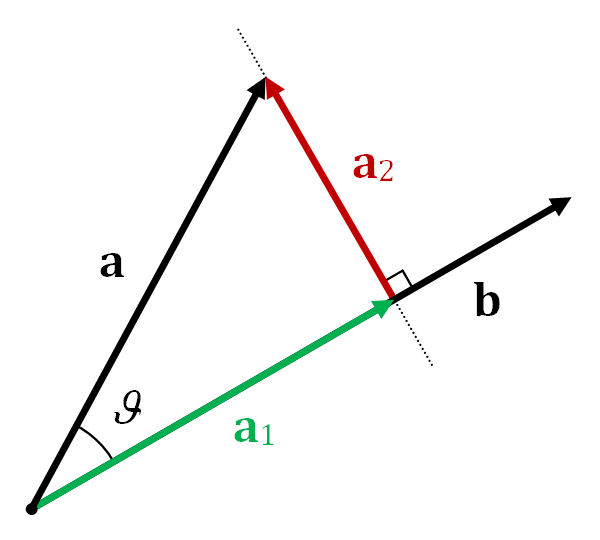
\includegraphics[height=3cm,width=1\textwidth,keepaspectratio]{Projection_and_rejection.png}
            \caption*{Projection of $\mathbf{a}$ on $\mathbf{b}$ ($\mathbf{a}_1$), and rejection of $\mathbf{a}$ from $\mathbf{b}$ ($\mathbf{a}_2$)}
            \label{fig:Projection_and_rejection.png}
        \end{figure}
    \end{column}
\end{columns}
\textbf{Where it can be used:}
\vspace{-0.5cm}
\begin{multicols}{2}
    \begin{itemize}
        \item Maps
        \item Blueprints
        \item Fitting algorithms (Least squares)
        \item Reduce matrix dimention
        \item RL fitness functions
    \end{itemize}
\end{multicols}
\end{frame}

\begin{frame}[t]{Projection 2D case from school}
\framesubtitle{Proofing 2d case formula (we project “b” on “a1”)}
    \begin{eqnarray}
        e = b-ax\\
        a_1 \cdot (b-a_1x)=0 \\ 
        a_1^T(b-a_1x)=0 \\
        a_1^Tb = a_1^Ta_1x \\ 
        \frac{a_1^Tb}{a_1^Ta_1}=x \text{ -- classic formula from school}
    \end{eqnarray}
    
\end{frame}

\begin{frame}[t]{Reference material}
    \framesubtitle{}
    \Large
    \begin{itemize}
        \item \href{https://www.youtube.com/watch?v=Y_Ac6KiQ1t0&list=PL49CF3715CB9EF31D&index=15}{Lecture 15 and 16}
        \item \textit{"Linear Algebra and Applications", pdf pages 181--204 }\\ Projections onto lines and Least squares
        \item \href{https://www.coursera.org/lecture/matrix-algebra-engineers/the-least-squares-problem-I56Qy}{The Least-Squares Problem}\\ Video from Matrix Algebra for Engineers course
        \item \href{https://matworld.ru/calculator/matrix-calculator-1.php}{Matrix online calculator}(russian)
    \end{itemize}
\end{frame}

\usebackgroundtemplate{}
\setbeamercolor{background canvas}{bg=}
% \includepdf[pages={2-7,10-11,18-20,23-27,29-34}]{class_5.pdf}

\fbckg{fibeamer/figs/last_page.png}
\frame[plain]{}

\end{document}